% copyright (c) 2018 Groupoid Infinity

\documentclass{article}
\usepackage{amscd}
\usepackage{listings}
\usepackage[numbers]{natbib}
\usepackage[only,llbracket,rrbracket,llparenthesis,rrparenthesis]{stmaryrd}
\usepackage{graphicx}
\usepackage{amsmath}
\usepackage{amssymb}
\usepackage{txfonts}
\usepackage{url}
\usepackage{tikz-cd}
\usepackage[utf8]{inputenc}

\newcommand*{\thead}[1]{\multicolumn{1}{c}{\bfseries #1}}

\usepackage{inconsolata}
\lstset{basicstyle=\small,inputencoding=utf8}

\begin{document}

\title{Mathematical Components for Cubical Syntax}
\author{Maksym Sokhatskyi $^1$ and Pavlo Maslianko $^1$}
\date{
    $^1$ National Technical University of Ukraine \\
    \small Igor Sikorsky Kyiv Polytechnical Institute\\
    \today
}

\maketitle

\begin{abstract}

The introduction of path spaces and its eliminators in cubical type theory (CTT)
as core type checker primitives calls for re-examination the proofs for mathematical components
in base libraries of the major provers Coq, Agda, F*, Lean.
They provide successful interpretation of calculus of inductive constructions
with predicative hierarchies, however the homotopical foundation of CTT demonstrates
computational semantics of univalence axiom and different kind of proofs by using path
composition and kan filling operations.

We present a base library compatible with Cubical language \cite{Mortberg17}
with respect to both run-time types and its mathematical models.
This library is about to extract to run-time languages from cubical syntax.
The basic core of the library contains abstractions for Pi, Sigma and Path types,
prop, set, and groupoid hierarchy, fixpoint, control structures, recursion schemes,
algebraic hierarchy, and category theory.

Despite minimalistic cubical syntax lacks type classes we show the elegant
way of encoding type classes in cubical. Also, the minimalistic syntax
gives us a lightweight extension to the pure type system (PTS) core
and simple and more straightforward extraction to it for a subset of CTT programs.

This article demonstrates an approach of type refinement to create
the library where run-time types and its mathematical models can be
easily separated while remain fit each other.
So we cover here only models needed for modeling run-time theories
while touching homotopical and geometrical models left for further
articles, as for quotient sets, circle, sphere, h-pushout, truncations,
iso, univalence, and other HoTT types.
\\
\\
{\bf Keywords}: Formal Methods, Type Theory, Programming Languages,
          Theoretical Computer Science, Applied Mathematics,
          Cubical Type Theory, Martin-Löf Type Theory
\end{abstract}

\newpage
\tableofcontents

\newpage
\section{Intro}

Usually from the mathematical point of view there is no differences between
different syntactic proofs of the same theorem. However from programming point of view
we can think of code reuse and precisely defined math libraries that reduce
the overal code size and provide simplicity for operating complex
structures (most heavy one is categorical library). So in this work we will focus
on proper decoupling and more programming friendly base library still usable
for mathematicians.

{\bf Research object}. The homotopy type theory base libraries in
Agda \footnote{\url{https://github.com/HoTT/HoTT- Agda}},
Cubical\footnote{\url{https://github.com/mortberg/cubicaltt}},
Lean\footnote{\url{ https://github.com/gebner/hott3}}, and
Coq\footnote{\url{https://github.com/HoTT/HoTT}}.
While modern Lean and Agda has the cubical mode, Coq lacks the computational semantics of path primitives
while has HoTT library. In this article, we unveil the practical implementation of the
base library for cubical type checkers with respect to target run-time environments.

{\bf Research subject}. We will analyze the base library through the needs of particular features,
like basic theorems about MLTT (Pi, Sigma, Equ, HeteroEqu), run-time types and data
structures (Empty, Unit, Maybe, Nat, List, Either, Tuple), control structures and applicative programming
(Functor, CoFunctor, ContraFunctor, CoContraFunctor, Applicative, CoApplicative, Monad,
CoMonad, Inductive, CoInductive), algebra tower (Monoid, CMonoid, Group, AbGroup, Ring, AbRing),
and category theory (Category, Functor, Initial, Terminal, Adjoint).
We use Martin-Löf Type Theory as a subject and its extension with [0,1] interval --- CTT.

{\bf Research results}. Research result is presented as source code repository that can be used by
cubicaltt language and contains the minimal base library used in this article.
These primitives form a valuable part of base library, so this article could be
considered as an brief introduction to several topics: {\bf MLTT}, {\bf Runtime Types},
{\bf Control Structures},  {\bf Recursive Schemes},
{\bf Abstract Algebra}, {\bf Category Theory}.
But the library has even more modules, that
exceed the scope of this article so you may refer to source code
repository \footnote{\url{https://github.com/groupoid/infinity}}.
Also we created a web page that can easily be read with phone \footnote{\url{https://groupoid.space/mltt/types}}.

We redefined the Cubical Syntax in LALR grammar and implented
syntax extension for Erlang language \footnote{\url{https://github.com/groupoid/infinity/blob/master/src/cub_parser.yrl}}.
If possible terms could be exracted
to Om syntax \footnote{\url{https://github.com/groupoid/om/blob/master/src/om_parse.erl}}.

All terms in this article will be given in this syntax.
The BNF notation consist of: 1) telescopes (contexts or sigma chains);
2) inductive data definitions (sum chains); 3) split eliminator;
4) branches of split eliminators; 5) pure dependet type theory syntax.
It also has where, import, module constructions.

\newpage
\begin{lstlisting}[mathescape=true]
     0 := #empty         imp    := [ ${\bf import}$ id ]
   brs := 0 + cobrs      tele   := 0 + cotele
   app := exp exp        cotele := ( exp : exp ) tele
    id := [ #nat ]       sum    := 0 + id tele + id tele | sum
   ids := [ id ]         br     := ids $\rightarrow$ exp
 codec := def dec        mod    := ${\bf module}$ id ${\bf where}$ imp def
   dec := 0 + codec      cobrs  := | br brs
   def := ${\bf data}$ id tele = sum + id tele : exp = exp + id tele : exp ${\bf where}$ def
   exp := cotele * exp + cotele $\rightarrow$ exp + exp $\rightarrow$ exp + app + ( exp ) + id +
          ${\bf split}$ cobrs + exp ${\bf .1}$ + exp ${\bf .2}$ + \cotele $\rightarrow$ exp
\end{lstlisting}

\subsection*{Types Taxonomy}

Types taxonomy shows us the core types categorized by a several axis:
1) dependent (D) and non-dependent (ND) terms;
2) recursive trees (R) or non-recursive (NR) data types;
3) inductive (+) or coinductive (*) types.

\begin{table}[h]
\centering
\caption{Types Taxonomy}
\label{tab:a}
\tabcolsep7pt
\begin{tabular}{lcccc}
\hline
\thead{NR+ND} & \thead{R+ND} & \thead{NR+D} & \thead{R+D}\\
\hline
unit        & nat    & pi      & vector \\
bool        & list   & circle  & fin \\
either      & path   & I       &  \\
maybe       &        &         &  \\
empty       &        &         &  \\
\hline
\thead{NR*ND} & \thead{R*ND} & \thead{NR*D} & \thead{R*D}\\
\hline
setoid      & stream & sigma   & cat  \\
functor     &        & equiv   & prop \\
applicative &        & iso     & set  \\
monad       &        & fiber   & groupoid \\
\end{tabular}
\end{table}


This library is dedicated to type checkers with cubical syntax,
based on interval [0,1] and MLTT as a core.
Please refer to original paper of cubicaltt \cite{Mortberg17}
which also given in the footnote \footnote{\url{http://www.cse.chalmers.se/~coquand/cubicaltt.pdf}}.
The base library is founded on top of cubical modules each
fall into one of the following categories:

(i) MLTT Types: {\bf pi}, {\bf sigma}, {\bf path};
(ii) Set Theory: {\bf prop}, {\bf set}, {\bf ordinal}, {\bf hedberg};
(iii) Run-Time Inductive Types: {\bf proto}, {\bf maybe}, {\bf bool}, {\bf nat}, {\bf list}, {\bf stream}, {\bf vector};
(iv) Abstract Algebra in {\bf algebra} module;
(v) Control Structures in {\bf control} module;
(vi) Recursion Schemes in {\bf recursion} module;
(vii) Category Theory: {\bf cat}, {\bf fun}, {\bf sip}, {\bf cones}, {\bf adj};
(viii) Univalent Foundations: {\bf equiv}, {\bf retract}, {\bf iso}, {\bf iso\_pi}, {\bf iso\_sigma}, {\bf univ};
(ix) Higher Inductive Types: {\bf interval}, {\bf circle}, {\bf pushout}, {\bf suspension}, {\bf quotient}, {\bf trunc}.
(x) Process Calculus in {\bf process} module;
(xi) Categories with Families: {\bf cwf}, {\bf csystem};
(xii) Type Checker will be in {\bf infinity} module.

This library is best to read guided by HoTT book \cite{HoTT}.
We tried to make it definitionally compatible with
the contemporary math foundations.

\section{Martin-Löf Type Theory}

As Martin-Löf Type Theory is used as modeling language,
the base library should include its definition and theorems.
The {\bf mltt} module contains the theorems of operational semantics of
dependent type theory and MLTT model, while {\bf cwf} and {\bf csystem}
modules contain its categorical semantics.

\subsection{Pi and Sigma}

Pi and Sigma modules provide basic theorems about dependent products and sum.
Here is tautology alias definitions for better syntax understanding.
In run-time Sigma is being transformed into pair and lambda into functions.
All type annotations and term dependence information are being erased.
Basic Pi and Sigma definitions are given in {\bf pi} and {\bf sigma} modules.

\begin{lstlisting}[mathescape=true]
Pi     (A:U) (B:A->U): U = (x:A) -> B(x)
lambda (A:U) (B:A->U) (a:A) (b:B(a)): A->B(a) = \ (x:A)->b
app    (A:U) (B:A->U) (a:A) (f:A->B(a)): B(a) = f(a)
Sigma  (A:U) (B:A->U): U = (x:A) * B(x)
pair   (A:U) (B:A->U) (a:A) (b:B(a)): Sigma A B = (a,b)
pr1    (A:U) (B:A->U) (x:Sigma A B): A = x.1
pr2    (A:U) (B:A->U) (x:Sigma A B): B (pr1 A B x) = x.2
\end{lstlisting}

Dependent functional extensionality.

\begin{lstlisting}[mathescape=true]
piExt (A: U) (B: A -> U) (f g: (x:A) -> B x)
      (p: (x:A) -> Path (B x) (f x) (g x))
    : Path ((y:A) -> B y) f g = <i> \(a: A) -> (p a) @ i
\end{lstlisting}

Induction principle for Sigma types.

\begin{lstlisting}[mathescape=true]
sigRec (A:U) (B:A -> U) (C:U)
       (g: (x:A) -> B(x) -> C) (p: Sigma A B)
     : C = g p.1 p.2
sigInd (A:U) (B:A -> U) (C: Sigma A B -> U)
       (p: Sigma A B) (g:(a:A)(b:B(a)) -> C(a,b))
     : C p = g p.1 p.2
\end{lstlisting}

Constructive version of Choice Axiom.

\begin{lstlisting}[mathescape=true]
ac   (A B: U) (R: A -> B -> U):
     (p: (x:A)->(y:B)*(R x y)) -> (f:A->B)*((x:A)->R(x)(f x))
  = \(g: (x:A)->(y:B)*(R x y)) -> (\(i:A)->(g i).1,\(j:A)->(g j).2)
\end{lstlisting}

\subsection{Identity Type}

Identity types or Prop types (when using PTS and built-in definitional equality for type checking
normalized term forms with means of identity) are both considered to be erased in run-time.
For modeling propositional equality later in 1984 was introduced Equ type. \cite{Lof84}
However unlike Pi and Sigma the eliminator J of Equ type is
not derivable in MLTT \cite{Hofmann96, Mortberg17, HoTT}.
Here we give the constructive J definition in CTT. Basic laws of Identity Type
are given in {\bf proto\_path} module.

\begin{lstlisting}[mathescape=true]
Path     (A: U) (a b: A): U
singl    (A: U) (a: A): U = (x: A) * Path A a x
refl     (A: U) (a: A): Path A a a
sym      (A: U) (a b: A) (p: Path A a b): Path A b a
eta      (A: U) (a: A): singl A a
contr    (A: U) (a b: A) (p: Path A a b): Path (singl A a) (eta A a) (b,p)
cong   (A B: U) (f: A->B) (a b: A) (p: Path A a b): Path B (f a) (f b)
subst    (A: U) (P: A->U) (a b: A) (p: Path A a b) (e: P a): P b
J        (A: U) (a: A) (C: (x: A) -> Path A a x -> U)
      (d: C a (refl A a)) (x: A) (p: Path A a x): C x p
   = subst (singl A a) T (eta A a) (x, p) (contr A a x p) d
           ${\bf where}$ T (z: singl A a): U = C (z.1) (z.2)
\end{lstlisting}

We can build setoid \cite{Bishop67} definition using sym, refl and cong which
represent symmetry, reflexivity and congruence.
Singleton is defined as Sigma with Path theorem. Contractability of singletons,
substitution and transport is used for proving the J eliminator \cite{HoTT}.

\subsection{$\infty$-Groupoid and h-Types}

The reasoning about higher equalties is made through explicit recursion.
We encode the level of path dimention through embedded natural numbers in the definition.

\begin{lstlisting}[mathescape=true]
${\bf data}$ N = Z | S (n: N)
\end{lstlisting}

As foundation we provide recursive and corecursive versions of groupoid definitions.
h-Types \cite{HoTT} (Prop, Set, Groupoid, etc) are defined through these primitives.

\begin{lstlisting}[mathescape=true]
n_grpd (A: U) (n: N): U = (a b: A) -> rec A a b n ${\bf where}$
   rec (A: U) (a b: A): (k: N) -> U
     = ${\bf split}$ { Z -> Path A a b ; S n -> n_grpd (Path A a b) n }
\end{lstlisting}

\begin{lstlisting}
inf_grpd (A: U): U
       = (carrier: A)
       * (eq: (a b: A) -> Path A a b)
       * ((a b: A) -> inf_grpd (Path A a b))
\end{lstlisting}

As you can see, h-Types properties are just eliminated recursors.

\begin{lstlisting}[mathescape=true]
isContr     (A: U): U = (x: A) * ((y: A) -> Path A x y)
isProp      (A: U): U = n_grpd A Z
isSet       (A: U): U = n_grpd A (S Z)
isGroupoid  (A: U): U = n_grpd A (S (S Z))
isGrp2      (A: U): U = n_grpd A (S (S (S Z)))
isGrp3      (A: U): U = n_grpd A (S (S (S (S Z))))
...
isInfinityGroupoid (A: U): U = inf_grpd A
\end{lstlisting}

And finally the definitions as refined h-Types through its properties.

\begin{lstlisting}[mathescape=true]
PROP         : U = (X:U) * isProp(X)
SET          : U = (X:U) * isSet(X)
GROUPOID     : U = (X:U) * isGroupoid(X)
INF_GROUPOID : U = (X:U) * isInfinityGroupoid(X)
\end{lstlisting}

The groupoids are defined in {\bf path} module.

\subsection{Operational Semantics}

By using such definition of MLTT we can commit the basic properties
of dependent theory, computational rules. The proofs are trivial
with {\bf refl} function and could be found in {\bf mltt} module.

\begin{equation} (\\(x:A) \rightarrow f(x))(a) = f(a) \end{equation}
\begin{equation} f = (\\(x:A) \rightarrow f(x)) \end{equation}
\begin{equation} pr_1 (a,b) = a \end{equation}
\begin{equation} pr_2 (a,b) = b \end{equation}
\begin{equation} (pr_1 p,pr_2 p) = p \end{equation}

Here is full list of inference rules properties.
We grouped them as in MLTT paper \cite{Lof84}. The system lack Nat and List
types as they can be church encoded.

\begin{lstlisting}[mathescape=true]
MLTT (A:U): U
  = (Pi_Former:  (A->U)->U)
  * (Pi_Intro:   (B:A->U) (a:A)->B a->(A->B a))
  * (Pi_Elim:    (B:A->U) (a:A)->(A->B a)->B a)
  * (Pi_Comp1:   (B:A->U) (a:A) (f:A->B a) -> Equ (B a)
                 (Pi_Elim B a (Pi_Intro B a (f a)))(f a))
  * (Pi_Comp2:   (B: A->U) (a:A) (f:A->B a) ->
                 Equ (A->B a) f (\(x:A)->Pi_Elim B a f))
  * (Sig_Former: (A->U)->U)
  * (Sig_Intro:  (B:A->U) (a:A)->(b:B a)->Sigma A B)
  * (Sig_Elim1:  (B:A->U)->(_: Sigma A B)->A)
  * (Sig_Elim2:  (B:A->U)->(x: Sigma A B)->B (pr1 A B x))
  * (Sig_Comp1:  (B:A->U) (a:A) (b: B a)->Equ A a
                 (Sigma_Elim1 B (Sigma_Intro B a b)))
  * (Sig_Comp2:  (B:A->U) (a:A) (b:B a)->Equ (B a) b
                 (Sigma_Elim2 B (a,b)))
  * (Id_Former:  A->A->U)
  * (Id_Intro:   (a:A) -> Equ A a a)
  * (Id_Elim:    (a x: A) (C: predicate A a)
                 (d:C a(Id_Intro a))(p:Equ A a x)->C x p)
  * (Id_Comp:    (x y:A)(C: D A)(p: Equ A x y)
                              (b: C x x (reflect A x))
                       (X: Equ U (C x x (reflect A x))
                                 (C x y p)) ->
                   HeteroEqu X b (J A x C b y p)) * Unit
\end{lstlisting}

Trivial check that our host type system preserves the dependent theory laws.
See computational rules in {\bf mltt} module.

\begin{lstlisting}[mathescape=true]
instance (A: U): MLTT A
  = ( Pi A, lambda A, app A, comp1 A, comp2 A,
      Sigma A, pair A, pr1 A, pr2 A, comp3 A, comp4 A, comp5 A,
      Equ A, reflect A, J A, comp6 A, tt )
\end{lstlisting}

\section{Runtime Types}

The purpose of run-time types is to build solid ground for
writing type checkers, evaluating results and printing models to console,
writing formally verified infinitely runned free comonadic processes.
In one framework we can combine the powerful semantics of CTT and
homotopical primitives to prove properties of run-time types in
a more simplier and elegant way.

\subsection{Proto}

The {\bf proto} module contains very basic common functions of id, composition and
synonims for intro and eliminators of Pi type, in dependent and non-dependent fasion.
Th {\bf proto} contains almost all short cuts to internal language constructions,
while {\bf pi} and {\bf sigma} modules contains only dependent versions.

\begin{lstlisting}[mathescape=true]
idfun    (A:U) (a:A): A = a
const  (A B:U) (a:B): A->B = \(_:A)->a
o    (A B C:U) (f: B->C) (g: A->B): A->C = \(x:A)->f(g(x))
\end{lstlisting}

\subsection{Empty and Unit}

The very basic types are empty type without elements and unit type with single element.
Interpreting types as propositions leads us to efq and neg eliminators of Empty type useful
for proving decidability, stablity and analogue of Hedberg theorem \cite{Hedberg98}.

\begin{lstlisting}[mathescape=true]
${\bf data}$ Empty =
emptyRec  (C: U): empty -> C = split {}
emptyInd  (C: empty->U): (z:empty) -> C z = ${\bf split}$ {}

${\bf data}$ Unit = tt
unitRec   (C: U) (x: C): unit -> C = ${\bf split}$ tt -> x
unitInd   (C: unit -> U) (x: C tt): (z:unit) -> C z = ${\bf split}$ tt -> x

efq        (A: U): Empty -> A = ${\bf split}$ {}
neg        (A: U): U = A -> Empty
dec        (A: U): U = either A (neg A)
stable     (A: U): U = neg (neg A) -> A
hedberg    (A: U) (h: (a x:A) -> stable (Path A a x)): isSet(A)
\end{lstlisting}

\subsection{Either and Tuple}

Either and Tuple are dual inductive data types.
They are  basic control structures and widely through all base library.
The tuple semantically same as both but is ready to pattern machthing.

\begin{lstlisting}[mathescape=true]
${\bf data}$ either (A B: U) = inl  (a: A) | inr (b: B)
${\bf data}$ tuple  (A B: U) = pair (a: A)       (b: B)

tupleRec  (A B C: U) (c: (x:A) (y:B) -> C)
        : (x: tuple A B) -> C
        = ${\bf split}$ pair a b -> c a b
tupleInd  (A B:U) (C: tuple A B -> U)
          (c: (x:A) (y:B) -> C(pair x y))
        : (x: tuple A B) -> C x
        = ${\bf split}$ pair a b -> c a b

eitherRec (A B C: U) (b: A -> C) (c: B -> C)
        : either A B -> C
        = ${\bf split}$ { inl x -> b(x) ; inr y -> c(y) }
eitherInd (A B: U) (C: either A B -> U)
          (x: (a: A) -> C (inl a))
          (y: (b: B) -> C (inr b))
        : (x: either A B) -> C x
        = ${\bf split}$ { inl i -> x i ; inr j -> y j }

\end{lstlisting}

\subsection{Bool}

The basic {\bf hedberg} theorem module could be used to prove that bool is set.
The {\bf bool} module is rarely used inside run-time library
however it is used is real world applications. Here we provide a proof
that bool is set by providing the proof that for any booleans path
between them is decidable.

\begin{lstlisting}[mathescape=true]
${\bf data}$ bool = false | true

a1: U = bool -> bool
a2: U = bool -> bool -> bool

negation: a1 = ${\bf split}$ { false -> true; true -> false}
or:  a2 = ${\bf split}$ { false->idfun bool;true->lambda bool(bool)true }
and: a2 = ${\bf split}$ { false->lambda bool(bool)false;true->idfun bool }

boolRec (A: U) (f t: A) : bool -> A = ${\bf split}$ { false -> f ; true -> t }
boolInd (A: bool -> U) (f: A false) (t: A true)
      : (n:bool) -> A n = split { false  -> f ; true -> t }

boolDec : (b1 b2: bool) -> dec (Path bool b1 b2)
boolSet : isSet bool = hedberg bool boolDec
\end{lstlisting}

\subsection{Maybe and Nat}

The {\bf maybe} and {\bf nat} modules are very useful for monadic protocol handling
and basic number processing. Nat data types is isomorphic
to infinite GMP positive integers of Erlang virtual machine.
Base library also include formal proof that fix maybe equals nat.
Maybe and Nat types are used in list library for handling special cases
of empty string and its length.

\begin{lstlisting}[mathescape=true]
${\bf data}$ maybe (A: U) = nothing | just (a: A)
${\bf data}$ nat          = zero    | succ (n: nat)

natRec (C:U) (z: C) (s: nat->C->C)
     : (n:nat) -> C
     = split { zero -> z ; succ n -> s n (natRec C z s n) }
natInd (C:nat->U) (z: C zero) (s: (n:nat) -> C(n) -> C(succ n))
     : (n:nat) -> C(n)
     = split { zero -> z ; succ n -> s n (natInd C z s n) }

maybeRec (A P: U) (n: P) (j: A->P)
       : maybe A->P = split { nothing -> n; just a -> j a}
maybeInd (A: U) (P: maybe A -> U) (n: P nothing) (j: (a: A) -> P (just a))
       : (a: maybe A) -> P a = split { nothing -> n ; just x -> j x }
\end{lstlisting}

Also we provide constructive proof that $Fix(Maybe) = Nat$.

\subsection{List and Stream}

The {\bf list} module implemented as very simple data type but no simplier
than needed to implement the type checker. List data type is
used to model categorical semantics of dependent type theory
as Categories with Famalies by Dybjer in {\bf cwf} module.
At the rest list has pretty standard implementation.

\begin{lstlisting}[mathescape=true]
${\bf data}$ list (A: U) = nil | cons (a: A) (as: list A)
null      (A: U): list A -> bool
head      (A: U): list A -> maybe A
tail      (A: U): list A -> maybe (list A)
nth       (A: U): nat -> list A -> maybe A
append    (A: U): list A -> list A -> list A
reverse   (A: U): list A -> list A
map     (A B: U): (A -> B) -> list A -> list B
zip     (A B: U): list A -> list B -> list (tuple A B)
foldr   (A B: U): (A -> B -> B) -> B -> list A -> B
switch    (A: U): (Unit -> list A) -> bool -> list A
filter    (A: U): (A -> bool) -> list A -> list A
length    (A: U): list A -> nat
\end{lstlisting}

The {\bf stream} module provide model for infinity streams, IO, and other corecursive models,
provide basic theorems about streams bisimulation (equality).

\begin{lstlisting}[mathescape=true]
${\bf data}$ stream (A: U) = cons (x: A) (xs: stream A)

tail      (A: U): stream A -> stream A
head      (A: U): stream A -> A
fib   (a b: nat): stream nat
seq (start: nat): stream nat

${\bf data}$ Bisimilar (A: U) (xs ys: stream A) =
     bisimilar (h: Path A (head A xs) (head A ys))
          (t: Bisimilar A (tail A xs) (tail A ys))

bisimilarityIsEquality (A: U) (xs ys: stream A):
     Path U (Bisimilar A xs ys) (Path (stream A) xs ys)
\end{lstlisting}

\subsection{Vector and Fin}

Vector and Fin are basic dependent inductive types. Fin types is used
in several models, e.g. for naming type constructors in the de Brujin fashion.

\begin{lstlisting}[mathescape=true]
${\bf data}$ vector (A:U)(n:nat) = vnil  | vcons (x:A)(xs:vector A (pred n))
${\bf data}$ fin         (n:nat) = fzero | fsucc (pre: fin (pred n))
\end{lstlisting}

Cubical Syntax lacks of full GADT support, so we need to ban using
type constructors and provide its typeable versions:

\begin{lstlisting}[mathescape=true]
fz (n: nat): Fin (succ n)          = fzero
fs (n: nat): Fin n -> Fin (succ n) = \(x: Fin n) -> fsucc x
\end{lstlisting}

\subsection{IO and Infinity IO}

We extracted the pure function for the following IO free structure
that encode the two functions for reading and printing string values in Church encoding.
The demonstarted program could be seen in Om project \footnote{\url{https://github.com/groupoid/om/blob/master/priv/normal/Morte/recursive}}.

\begin{lstlisting}[mathescape=true]
${\bf data}$ IO (A: U)
   = getLine (fun: String -> IO A)
   | putLine (io: IO A) (str: String)
   | pure (finish: A)

main: U = replicateM 100 (>>= String () getLine putLine)
\end{lstlisting}

The infinity IO sample is also provided by Om project \footnote{\url{https://github.com/groupoid/om/blob/master/priv/normal/Morte/corecursive}}
ans demonstrate the cofree comonadic encoding of process running.

\begin{lstlisting}[mathescape=true]
${\bf data}$ IOI.F (A State: U)
   = getLine: (fun: String -> State)
   | putLine: (str: String) (state: State)
   | pure: (finish: A)
\end{lstlisting}
\begin{lstlisting}[mathescape=true]
${\bf data}$ IOI (A State: U) =
     intro: (init: State)
            (action: State -> IOI.F A State)
\end{lstlisting}

We put Erlang Coinductive Bindings as pure function to comonad instance:

\begin{lstlisting}[mathescape=true]
copure()    -> fun (_) -> fun (IO) -> IO end end.
cogetLine() -> fun(IO) -> fun(_) ->
               L = ch:list(io:get_line("> ")),
               ch:ap(IO,[L]) end end.
coputLine() -> fun (S) -> fun(IO) ->
               X = ch:unlist(S),
               io:put_chars(": "++X), corec() end end.
corec()     -> ap('Morte':corecursive(),
               [copure(),cogetLine(),coputLine(),copure(),list([])]).
\end{lstlisting}

Extract the Erlang program from Abstract Syntax and run the program:

\begin{lstlisting}[mathescape=true]
> om_extract:extract("priv/normal/IOI"),  om:corec().
> 1
: 1
\end{lstlisting}

\section{Control Structures}

SKI combinatoric lambda caclulus was developed by Ukranian Logician
Moisei Isaievich Sheinfinkel. It could be used as basis for computational
foundation just like lambda caclulus. Later Connor McBride \cite{McBride08} evolved the SKI
into Applicative type-class. It is known that SKI is just an Church encoded Applicative.
Now Applicative type-class is a mandatory tool in any base library.
All control structures are given in {\bf control} module.

\begin{equation}
 S = apply : (x \rightarrow b \rightarrow c) \rightarrow (x \rightarrow b) \rightarrow (x \rightarrow c)
\end{equation}
\begin{equation}
 K = pure  : a \rightarrow (x \rightarrow a)
\end{equation}
\begin{equation}
 I = S K K
\end{equation}

We show here the developer's logic behind the scenes of implementation. First we need
to cut all basic type classes like Pure, Applicative, Functor, CoFunctor,
ContraFunctor, CoContraFunctor and their flip eliminators. Another powerful control
structure from came from Category Theory are Monad and CoMonad that is used
for modeling IO.

\subsection{Signatures}

Here is given all signatures supported in control base library, mainly functors and monads.

\begin{lstlisting}[mathescape=true]
pure_sig                   A  -> F A
extract_sig              F A  ->   A
extend_sig         (F A -> B) -> F A -> F B
appl_sig           F (A -> B) -> F A -> F B
fmap_sig             (A -> B) -> F A -> F B
unmap_sig        (F A -> F B) ->  (A -> B)
contra_sig           (B -> A) -> F A -> F B
uncontra_sig     (F A -> F B) ->  (B -> A)
cofmap_sig           (B -> A) -> F B -> F A
uncofmap_sig     (F B -> F A) ->  (B -> A)
cocontra_sig         (A -> B) -> F B -> F A
uncocontra_sig   (F B -> F A) ->  (A -> B)
join_sig              F (F A) -> F A
dup_sig                  F A  -> F (F A)
bind_sig            F A ->(A  -> F B)-> F B
\end{lstlisting}

The we build up a signatures of type clases build as sigma encoded contexts or telescopes.
The signatures are made external for code compactification.
Then we select $F: U \rightarrow U$ functor as common head for sigma types.
All quantifiers for members and laws are carried within projections.
Projections contains full signature except F. These types could be considered for run-time.
Also you may read Oleg Kiselev Type-Classes in ML. \footnote{\url{http://okmij.org/ftp/Computation/typeclass.html}}
Here is we encode type-classes with Sigma and instances with nested tuples.

\subsection{Run-time types}

Coupling signatures with type-class parameters gives us a notion of run-time types.
All type-value projections along with parameters are being erased during code extraction.

\begin{lstlisting}[mathescape=true]
pure:        U = (F:U->U) *     pure_sig F
functor:     U = (F:U->U) *     fmap_sig F
applicative: U = (F:U->U) * (_: pure_sig F)
                          * (_: fmap_sig F)
                          * (   appl_sig F)

monad: U = (_: applicative)
         * (   bind_sig F.1)
\end{lstlisting}

\subsection{Accessors}

Accessors are common technique in Type Refinement approach for beautifying the code.
As cubical syntax provide only .1 and .2 notion for projections it is good to have
named field accessors for all projections.

\begin{lstlisting}[mathescape=true]
fmap (a: functor):     fmap_sig a.1 = a.2
pure (a: applicative): pure_sig a.1 = a.2.1
amap (a: applicative): fmap_sig a.1 = a.2.2.1
ap   (a: applicative): appl_sig a.1 = a.2.2.2
\end{lstlisting}

\subsection{Theorems as Proof-carrying Code}

The formal definition of control structures comes in Type Refinement approach when
we separate the algebraic structure and its properties.

\subsection*{Functor}

Such we defined the functor as $\Sigma_{F:U->U} fmap_F$. And the Functor has two laws:

\begin{equation} o(fmap,id) = id \end{equation}
\begin{equation} fmap(o(g,h)) = o(fmap(g),fmap(h)) \end{equation}

\begin{lstlisting}[mathescape=true]
isFunctor (F: functor): U
    = (id: (A: U) -> (x: F.1 A) ->
           Path (F.1 A) x ((fmap F) A A (idfun A) x))
    * (compose: (A B C:U) (f:B->C) (g:A->B) (x:F.1 A) ->
      Path (F.1 C) (F.2 A C (o A B C f g) x)
       ((o (F.1 A) (F.1 B) (F.1 C)
           (F.2 B C f) (F.2 A B g)) x)) * Unit
\end{lstlisting}

\subsection*{Applicative}

Being applicative property contains applicative laws:

\begin{equation} ap(pure(id),x) = id(x) \end{equation}
\begin{equation} ap(pure(f),pure(x)) = pure(f(x)) \end{equation}
\begin{equation} ap(ap(ap(pure(o),u),v),w) = ap(u,ap(v,w)) \end{equation}
\begin{equation} ap(u,pure(y)) = ap(pure(\\f.f(y)),u) \end{equation}

\begin{lstlisting}[mathescape=true]
isApplicative (F: applicative): U
    = (id:  (A:U) -> (x: F.1 A) ->
       Path (F.1 A) x (ap F A A (pure F (id A) (idfun A)) x))
    * (hom: (A B:U)(f:A->B)(x: A) ->
       Path (F.1 B) (pure F B (f x))
                    (ap F A B (pure F (A->B) f) (pure F A x)))
    * (cmp: (A B C:U)(v: F.1(A->B))(u:F.1(B->C))(w:F.1 A) ->
       Path (F.1 C) (ap F B C u (ap F A B v w))
                    (ap F A C (ap F (A->B) (A->C)
                              (ap F (B->C) ((A->B)->(A->C))
                    (pure F (ot A B C) (o A B C)) u) v) w))
    * (xchg: (A B:U)(x:A)(u:F.1(A->B))(f:A->B) ->
       Path (F.1 B) (ap F A B u ((pure F) A x))
                    (ap F (A->B) B (pure F ((A->B)->B)
                                   (\(f:A->B)->f(x))) u)) * Unit
\end{lstlisting}

Then we can define the FUNCTOR as Sigma of fuctor signature and functor properties:

\begin{lstlisting}[mathescape=true]
FUNCTOR:     U = (f: functor) * isFunctor f
APPLICATIVE: U = (f: applicative)
               * (_: isFunctor (f.1,f.2.2.1))
               * isApplicative f
\end{lstlisting}
\begin{lstlisting}[mathescape=true]
MONAD: U = (f: monad)
       * (_: isFunctor (f.1,f.2.2.1))
       * (_: isApplicative (f.1,f.2.1,f.2.2.1,f.2.2.2.1))
       * isMonad f
\end{lstlisting}

We do not show here the full Control library (only the Functor and Applicative instances)
due to sizes of the terms. Here is sample list functor instance defined in {\bf list\_theory} module.

\begin{lstlisting}[mathescape=true]
functorlist: functor = (list,map)
functorlaws: FUNCTOR  = ((list,map),(list_id,list_compose,tt))
\end{lstlisting}

\section{Recursion Schemes}

A F-algebras provide us a generalized notion of folds over a parametrized inductive structures \cite{Pfenning89}.
The formalism of recursion schemes was developed by Varmo Vene and Nicola
Gambino \cite{Gambino04, Vene00} and categorically by Bart Jacobs, Henning Basold
and Herman Geuvers \cite{Jacobs97, Basold16}.
Recursion Schemes, Fixpoint, Free and CoFree protocol data types are defined in {\bf recursion} module.
It contains: Ana, Cata, Para, Hylo, Zygo, PrePro, PostPro, Apo, Gapo, Futu,
Histo, Chrono, Mutu, Meta, MCata, Inductive and CoInductive definitions.

The core notion for recursion schemes are F-algebras. $(\mu F, in)$ is the initial F-algebra if for any F-algebra $(C, \varphi)$
there exists a unique arrow $\llparenthesis \varphi \rrparenthesis : \mu F \rightarrow C$ where $f = \llparenthesis \varphi \rrparenthesis$
and is called catamorphism. Similar a F-coalgebra $(\nu F, out)$ is the terminal
F-coalgebra if for any F-coalgebra $(C, \varphi)$ there exists unique arrow
$\llbracket \varphi \rrbracket : C \rightarrow \nu F$ where $f =
\llbracket \varphi \rrbracket$

\begin{center}
\begin{tabular}{lcl}
\begin{tikzcd}
F\ \mu F \arrow{d}[left]{F\ \llparenthesis \varphi \rrparenthesis} \arrow{r}{in} & \mu F \arrow{d}{\llparenthesis \varphi \rrparenthesis} \\
F C \arrow{r}{\varphi} & C \end{tikzcd} & & \begin{tikzcd}
C \arrow{d}[left]{ \llbracket \varphi \rrbracket} \arrow{r}{\phi} & F\ C\arrow{d}{F\ \llbracket \varphi \rrbracket} \\
\nu F \arrow{r}{out} & F \nu F\end{tikzcd} \\
\ & \  &\  \\
$f \circ in = \varphi \circ F\ f \equiv f = \llparenthesis \varphi \rrparenthesis$& &
$out \circ f = F\ f \circ \varphi \equiv f = \llbracket \varphi \rrbracket$ \\
\end{tabular}
\end{center}

\subsection{Fixpoint and Free Structures}

The Fixpoint recursive data type has two eliminators: in and out.
The $\mu$ and $\nu$ data types define the A+F(B) and A*F(B) non-recursive
inductive and coinductive type respectively.

Free and Cofree represent terminated or non-terminated sequence of functorial
bindings defined as $\mu x . a + f x$ and $\nu x . a * f x$ where $\mu < fix < \nu$.
Also we defined unpacking routines for fix and for (co-)free structures.

\begin{lstlisting}[mathescape=true]
${\bf data}$ fix (F:U->U)= Fix (point: F (fix F))
out (F:U->U): fix F -> F (fix F) = ${\bf split}$ Fix f -> f
in  (F:U->U): F (fix F) -> fix F = \(x: F (fix F)) -> Fix x
\end{lstlisting}
\begin{lstlisting}[mathescape=true]
${\bf data}$ mu (F:U->U) (A B:U) = Return (a: A) | Bind (f: F B)
${\bf data}$ nu (F:U->U) (A B:U) = CoBind (a: A) (f: F B)
${\bf data}$ free (F:U->U) (A:U) = Free (_: fix (mu F A))
${\bf data}$ cofree (F:U->U) (A:U) = CoFree (_: fix (nu F A))
unfree (F:U->U) (A:U): free F A -> fix (mu F A)
uncofree (F:U->U) (A:U): cofree F A -> fix (nu F A)
\end{lstlisting}

\subsection{Catamorphism and Futumorphism}

Catamorphism denotes the homomorphism from initial algebra to some other algebras.
A generalization of folds.

\begin{lstlisting}[mathescape=true]
cata (A: U) (F: functor) (alg: F.1 A -> A) (f: fix F.1): A
   = alg (F.2 (fix F.1) A (cata A F alg) (out_ F.1 f))
\end{lstlisting}

Histomorphism is a recursion based on a recursive cofree structure with unpacking control.
A generalization of cata

\begin{lstlisting}[mathescape=true]
histo (A:U) (F: functor)
      (f: F.1 (cofree F.1 A) -> A) (z: fix F.1): A
  = extract A ((cata (cofree F.1 A) F (\(x: F.1 (cofree F.1 A)) ->
    CoFree (Fix (CoBind (f x) ((F.2 (cofree F.1 A)
    (fix (nu F.1 A)) (uncofree F.1 A) x)))))) z) ${\bf where}$
  extract (A: U): cofree F.1 A -> A = ${\bf split}$
    CoFree f -> unpack_fix f ${\bf where}$
  unpack_fix: fix (nu F.1 A) -> A = ${\bf split}$
    Fix f -> unpack_cofree f ${\bf where}$
  unpack_cofree: nu F.1 A (fix (nu F.1 A)) -> A = ${\bf split}$
    CoBind a -> a
\end{lstlisting}

\subsection{Anamorphism and Histomorphism}

Anamorphism denotes the homomorphism to terminal coalgebra of an endofunctor
from some other coalgebras. A generalization of unfolds.

\begin{lstlisting}[mathescape=true]
ana (A: U) (F: functor) (coalg: A -> F.1 A) (a: A): fix F.1
  = Fix (F.2 A (fix F.1) (ana A F coalg) (coalg a))
\end{lstlisting}

Futumorphism is a recursion based on a recursive free structure with unpacking control.
A generalization of anamorphisms.

\begin{lstlisting}[mathescape=true]
futu (A: U) (F: functor)
     (f: A -> F.1 (free F.1 A)) (a: A): fix F.1
  = Fix (F.2 (free F.1 A) (fix F.1) (\(z: free F.1 A) -> w z) (f a)) ${\bf where}$
  w: free F.1 A -> fix F.1 = ${\bf split}$
    Free x -> unpack_fix x ${\bf where}$
  unpack_free: mu F.1 A (fix (mu F.1 A)) -> fix F.1 = ${\bf split}$
    Return x -> futu A F f x
    Bind g -> Fix (F.2 (fix (mu F.1 A)) (fix F.1)
                        (\(x: fix (mu F.1 A)) -> w (Free x)) g)
  unpack_fix: fix (mu F.1 A) -> fix F.1 = ${\bf split}$
    Fix x -> unpack_free x
\end{lstlisting}

\subsection{Inductive and Coninductive Types}

Inductive types are given as direct encoding of commutative square as in \cite{Wu13}.
For inductive and coinductive data types the first two fields of sigma are flipped.

\begin{lstlisting}[mathescape=true]
ind (A: U) (F: U -> U) : U
    = (in_: F (fix F) -> fix F)
    * (in_rev: fix F -> F (fix F))
    * (fold_: (F A -> A) -> fix F -> A)
    * (free_: (A -> F (free F A)) -> A -> fix F)
    * Unit

coind (A: U) (F: U -> U) : U
    = (out_: fix F -> F (fix F))
    * (out_rev: F (fix F) -> fix F)
    * (unfold_: (A -> F A) -> A -> fix F)
    * (cofree_: (F (cofree F A) -> A) -> fix F -> A)
    * Unit
\end{lstlisting}

The two instances with corresponding recursors is then given by recursion schemes.

\begin{lstlisting}[mathescape=true]
inductive (A: U) (F: functor): ind A F.1
    = (in_ F.1,out_ F.1,cata A F,futu A F,tt)
coinductive (A: U) (F: functor): coind A F.1
    = (out_ F.1,in_ F.1,ana A F,histo A F,tt)
\end{lstlisting}

Here is simple example how two instances (inductive and coinductive) of list could be defined.

\begin{lstlisting}[mathescape=true]
ind_list   (T:U): ind   list T = inductive   (list,map) T
coind_list (T:U): coind list T = coinductive (list,map) T
\end{lstlisting}

\section{Abstract Algebra}

Algebraic structures in {\bf algebra} are the natural math companion to
more developer oriented {\bf control} module, which is also sort of algebraic structures.
Here you can find everything except Fields and Modules yet. Only up to Abelian Groups and Rings.
However this structures is enough to define cagegories of Abelian groups and Grothendieck adjunctions.

\subsection{Monoid and Commutative Monoid}

The monoid is a simple algebra with one binary operation: M -> M -> M.
By definition monoid is associative and has left and right identities.
Commutative monoid is one predicate stronger, expects the operation
to be commutative.

\begin{lstlisting}[mathescape=true]
isAssociative (M: U) (op: M -> M -> M) : U

hasIdentity (M : U) (op : M -> M -> M) (id : M) : U
  = (_ : hasLeftIdentity M op id)
  * (hasRightIdentity M op id)
\end{lstlisting}

\begin{lstlisting}[mathescape=true]
isMonoid (M: SET): U
  = (op: M.1 -> M.1 -> M.1)
  * (_: isAssociative M.1 op)
  * (id: M.1)
  * (hasIdentity M.1 op id)
\end{lstlisting}

\begin{lstlisting}[mathescape=true]
isCMonoid (M: SET): U
  = (m: isMonoid M)
  * (isCommutative M.1 m.1)
\end{lstlisting}

\subsection{Group and Abelian Group}

Group is a Monoid with inverse morphisms.

\begin{lstlisting}[mathescape=true]
isGroup (G: SET): U
  = (m: isMonoid G)
  * (inv: G.1 -> G.1)
  * (hasInverse G.1 m.1 m.2.2.1 inv)
\end{lstlisting}

Abelian group is a commutative group with inverse morphisms.

\begin{lstlisting}[mathescape=true]
isAbGroup (G: SET): U
  = (g: isGroup G)
  * (isCommutative G.1 g.1.1)
\end{lstlisting}

\subsection{Ring and Abelian Ring}

Ring has two operations, one (*) is a Monoid and other (+) is an Abelian Group.
Ring is supposed to be distrubitive across (*) and (+) operations.

\begin{lstlisting}[mathescape=true]
isRing (R: SET): U
  = (mul: isMonoid R)
  * (add: isAbGroup R)
  * (isDistributive R.1 add.1.1.1 mul.1)
\end{lstlisting}

Abelian Ring is a Ring where (*) operation is commutative monoid.

\begin{lstlisting}[mathescape=true]
isAbRing (R: SET): U
  = (mul: isCMonoid R)
  * (add: isAbGroup R)
  * (isDistributive R.1 add.1.1.1 mul.1.1)
\end{lstlisting}

%\newpage
\section{Category Theory}

The general notion of category is given as in \cite{Shulman15} and \cite{HoTT}.
Usual notion of category is called precategory while category is saturated precategories.
The Category Theory consists of five modules: 1) {\bf cat} for precategory, category and (co-)terminal objects;
2) {\bf fun} for categorical functor, its instances (id, compose), coslice category construction,
universal arrows, and equivalence theorems; 3) {\bf sip} for structure definition and
structure identity principle theorem; 4) {\bf cones} for cones, pullback definitions, and theorems;
5) {\bf adj} for natural transformations and adjunctions. As a stress example for categorical library
we took the C-Systems model of Vladimir Voevodsky implemented in {\bf csystem} module on
top of our categorical library. C-Systems are a categorical model of dependent type theory,
similar to Dybjer's Categories with Families ({\bf cwf} module).

We divide the carrier and morphisms as algebraic structure of category
definition (in essense CT is an abstract algebra of functions) and laws (theorems
or categorical properies, defined as equalities on morphisms):

\begin{lstlisting}[mathescape=true]
cat: U = (A: U) * (A -> A -> U)
\end{lstlisting}

\subsection{Theorems}

We define theorems section as predicate in a form of Sigma
which is usual a carrier for theorems. More formal, precategory $A$ consists of the following:
(i)   A type $A_0$, whose elements are called objects. We write $a: A$ for $a: A_0$.
(ii)  For each $a,b: A$, a set $hom_A(a,b)$, whose elements are called arrows or morphisms.
(iii) For each $a: A$, a morphism $1_a : hom_A(a,a)$, called the identity morphism.
(iv)  For each $a,b,c: A$, a function $hom_A(b,c) \rightarrow hom_A(a,b) \rightarrow hom_A(a,c)$
      called composition, and denoted $g \circ f$.
(v)   For each $a,b: A$ and $f: hom_A(a,b)$, we have $f = 1_b \circ f$ and $f = f \circ 1_a$.
(vi)  For each $a,b,c,d: A$ and $f: hom_A(a,b)$, $g: hom_A(b,c)$, $h: homA(c,d)$,
      we have $h \circ (g \circ f ) = (h \circ g) \circ f$.

\begin{lstlisting}[mathescape=true]
isPrecategory (C: cat): U
  = (id:      (x: C.1) -> C.2 x x)
  * (c:       (x y z:C.1) -> C.2 x y -> C.2 y z -> C.2 x z)
  * (homSet:  (x y: C.1) -> isSet (C.2 x y))
  * (left:    (x y: C.1) -> (f: C.2 x y) ->
              Path (C.2 x y) (c x x y (id x) f) f)
  * (right:   (x y: C.1) -> (f: C.2 x y) ->
              Path (C.2 x y) (c x y y f (id y)) f)
  * (compose: (x y z w: C.1) -> (f: C.2 x y) ->
              (g: C.2 y z) -> (h: C.2 z w) ->
              Path (C.2 x w) (c x z w (c x y z f g) h)
              (c x y w f (c y z w g h))) * Unit

precategory: U = (C: cat) * isPrecategory C
\end{lstlisting}

\subsection{Accessors}

Due to the nature of minimalistic syntax for each algebraic structure
should be defined the accessors for its projections to avoid long projection
composition, e.g. 2.2.2.2.2.1.

\begin{lstlisting}[mathescape=true]
carrier (C: precategory): U = C.1.1
hom     (C: precategory) (a b: carrier C): U = C.1.2 a b
path    (C: precategory) (x: carrier C): hom C x x = C.2.1 x
compose (C: precategory) (x y z: carrier C) (f: hom C x y)
        (g: hom C y z): hom C x z = C.2.2.1 x y z f g
\end{lstlisting}

\subsection{Rezk Completion}

"Every fully faithful and essentially surjective functor
is an equivalence of categories" in classical set-based category
theory is equivalent to the axiom of choice.

(i) For strict categories, it is equivalent to to the axiom of choice.
(ii) For precategories, it is underivable.
(iii) For saturated categories, it is derivable without axiom of choice.

Anything we say about objects of a category is invariant under isomorphism.

\begin{lstlisting}
iso (C: precategory) (A B: carrier C): U
  = (f: hom C A B)
  * (g: hom C B A)
  * (_: Path (hom C A A) (compose C A B A f g) (path C A))
  * (   Path (hom C B B) (compose C B A B g f) (path C B))

isCategory (C: precategory): U
  = (A: carrier C) -> isContr ((B: carrier C) * iso C A B)

category: U = (C: precategory) * isCategory C
\end{lstlisting}

Such category saturation or competion is called Rezk competion \cite{Shulman15}.
Source code in Coq of Rezk competion for comparison could be taken here \footnote{\url{https://github.com/benediktahrens/rezk_completion/blob/master/precategories.v}}.

\subsection{Terminals and Cones}

Initiality and Terminality encoded directly from its definition.

\begin{lstlisting}[mathescape=true]
isInitial  (C: precategory) (x: carrier C): U
         = (y: carrier C) -> isContr (hom C x y)
isTerminal (C: precategory) (y: carrier C): U
         = (x: carrier C) -> isContr (hom C x y)

initial  (C: precategory): U = (x:carrier C) * isInitial C x
terminal (C: precategory): U = (y:carrier C) * isTerminal C y

hasCospanCone (C: precategory) (D: cospan C) (W: carrier C): U
  = (f : hom C W D.2.1.1)
  * (g : hom C W D.2.2.1)
  * Path (hom C W D.1) (compose C W D.2.1.1 D.1 f D.2.1.2)
                       (compose C W D.2.2.1 D.1 g D.2.2.2)

cospanCone (C: precategory) (D: cospan C): U
  = (W: carrier C)
  * hasCospanCone C D W
\end{lstlisting}

Cones and Pullback definitions, properties and theorems are in {\bf cones} module.

\subsection{Functors}

Categorical functor definition and instances are in {\bf fun} module.

\begin{lstlisting}[mathescape=true]
catfunctor (A B: precategory): U
  = (ob:   carrier A -> carrier B)
  * (mor:  (x y: carrier A) ->
           hom A x y -> hom B (ob x) (ob y))
  * (id:   (x: carrier A) ->
           Path (hom B (ob x) (ob x))
                (mor x x (path A x)) (path B (ob x)))
  * (cmp:  (x y z: carrier A) -> (f: hom A x y) -> (g: hom A y z) ->
           Path (hom B (ob x) (ob z)) (mor x z (compose A x y z f g))
           (compose B (ob x) (ob y) (ob z) (mor x y f) (mor y z g))) * Unit
\end{lstlisting}

\subsection{Natural Transformations and Andjunctions}

Natural Transformations and Adjunctions are defined in {\bf adj} module.

\begin{lstlisting}[mathescape=true]
isNaturalTrans (C D: precategory)
               (F G: catfunctor C D)
               (eta: (x: carrier C) -> hom D (F.1 x) (G.1 x)): U
  = (x y: carrier C) (h: hom C x y) ->
    Path (hom D (F.1 x) (G.1 y))
         (compose D (F.1 x) (F.1 y) (G.1 y) (F.2.1 x y h) (eta y))
         (compose D (F.1 x) (G.1 x) (G.1 y) (eta x) (G.2.1 x y h))
\end{lstlisting}

\begin{lstlisting}[mathescape=true]
ntrans (C D: precategory) (F G: catfunctor C D): U
  = (eta: (x: carrier C) -> hom D (F.1 x) (G.1 x))
  * (isNaturalTrans C D F G eta)
\end{lstlisting}

\begin{lstlisting}[mathescape=true]
adjoint (C D: precategory) (F: catfunctor D C) (G: catfunctor C D) : U
  = (unit: ntrans D D (idFunctor D) (compFunctor D C D F G))
  * (counit: ntrans C C (compFunctor C D C G F) (idFunctor C))
  * areAdjoint C D F G unit counit
\end{lstlisting}

\newpage
\subsection{Examples}

Here we give two complex examples that cover the usage of all categorical library (five modules)
and abstract {\bf algebra} module.

\subsubsection*{Grothendieck Adjoint}

The top level example of using universal {\bf algebra} module and categorical modules
is given as Grothendieck Adjoint in categories of Abelian groups {\bf Ab} and
commutative monoids {\bf CMon} of two functors: forgetful from, {\bf Ab} to {\bf CMon}; and
Grothendieck, from {\bf CMon} to {\bf Ab}.

\begin{lstlisting}[mathescape=true]
Ab:   precategory = ((abgroup,abgrouphom),(id,c,HomSet,L,R,C)) ...
CMon: precategory = ((cmonoid,cmonoidhom),(id,c,HomSet,L,R,C)) ...

grothendieck: catfunctor CMon Ab = ...
forgetful:    catfunctor Ab CMon = ...

grothendieck_adjoint: adjoint Ab CMon grothendieck forgetful
  = transport (<i> adjoint Ab CMon (gro_ifeq @ i) forgetgul)
              (univarr_adjoint CMon Ab forgetful gro_univarr)
\end{lstlisting}

\subsubsection*{C-Systems}

In the {\bf csystem} module you can find a proof that
Universe Category is enough to define the C-System.

\newpage
\section{Conclusion}

We finished the story about Groupoid Infinity base library.
Despite we were limited with paper size and could not cover
homotopical types and other run-time types, we tried to put
into overview the very strong core of the base library by
providing different sections of modules:
1) MLTT Core Types; 2) Run-time Types; 3) Control Structures;
4) Recursion Schemes; 5) Abstract Algebra; 6) Category Theory.

\begin{figure}[h]
  \centerline{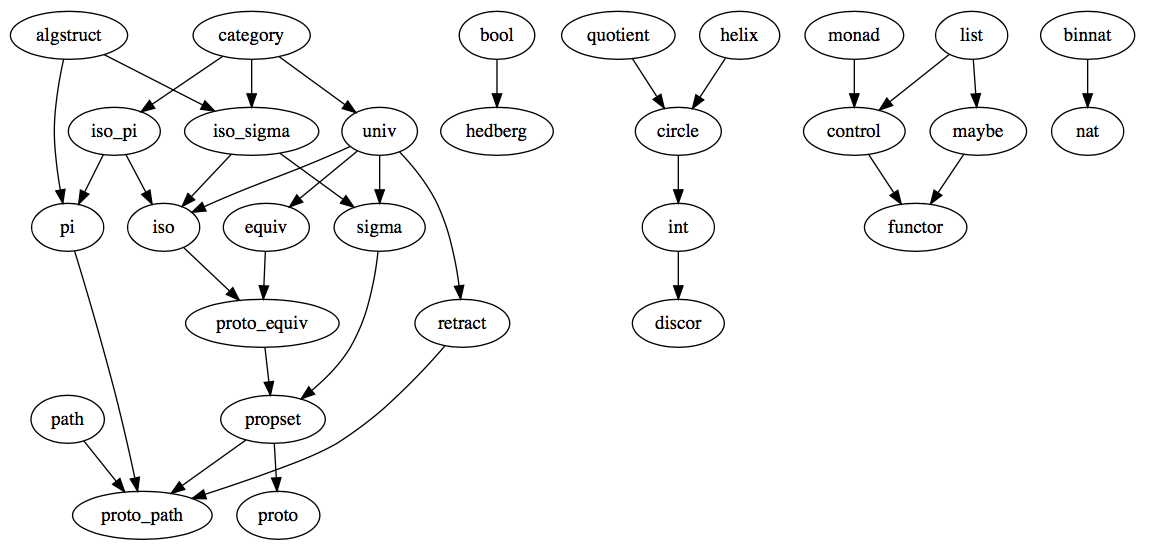
\includegraphics[scale=0.20]{baselib}}
  \caption{Base library and its dependencies}
\end{figure}

In other articles there will be coverage of the folliwing sections of modules:
1) Process Calculus; 2) Univalent Foundations; 3) Categories with Families;
4) Higher Inductive Types.
The main advantage of our mathematical components design
was motivated and driven by simplicity and clarity, having complete
and readable predicative definitions. The minimized Cubical
Syntax refined for our purposes covers most of the run-time
library which is a major part of the work.

\begin{table}[h]
\centering
\caption{Base Library defined in article}
\label{tab:a}
\tabcolsep7pt
\begin{tabular}{lcccccc}
\hline
\thead{Module}&\thead{LOC}&\thead{Module}&\thead{LOC}&\thead{Module}&\thead{LOC} \\
\hline
{\bf algerbra} & 360 & {\bf fun}         & 212 & {\bf cat}       & 59  \\
{\bf adj}      & 72  & {\bf csystem}     & 508 & {\bf hedberg}   & 28  \\
{\bf list}     & 63  & {\bf maybe}       & 19  & {\bf mltt}      & 55  \\
{\bf nat}      & 65  & {\bf path}        & 39  & {\bf pi}        & 15  \\
{\bf proto}    & 20  & {\bf proto\_path} & 16  & {\bf recursion} & 98  \\
{\bf sip}      & 166 & {\bf sigma}       & 36  & {\bf stream}    & 10  \\
{\bf cones}    & 109 & {\bf control}     & 71  & {\bf bool}      & 11  \\
\hline
\end{tabular}
\end{table}

The library consists of highly decoupled modules. E.g. we shown that we can combine
Abstract Algebra onbjects with Category Theory and created new Categories.
The models are given almost in pure MLTT with explicit notion of all types used
for term definition. In that way this kind of specification avoid a class of mistakes
connected with implicit specifications hidden inside type checker.
The library doesn't stop evolving with this report and will evolve with more
complex powerful theories remaining comfortable for run-time code extraction
to Erlang\footnote{https://erlang.org}.

\newpage
\bibliographystyle{plain}
\bibliography{types}

\end{document}

